\documentclass{amsart}

\usepackage[english]{babel}
\usepackage[utf8]{inputenc}
\usepackage{graphicx}
\usepackage{mathtools}
\usepackage{amsthm}
\usepackage{amsfonts}
\usepackage{hyperref}
\usepackage[singlelinecheck=false]{caption}
\usepackage{enumitem}
\usepackage[justification=centering]{caption}
\usepackage{indentfirst}
\usepackage{listings}

\makeatletter
\def\subsection{\@startsection{subsection}{3}%
  \z@{.5\linespacing\@plus.7\linespacing}{.1\linespacing}%
  {\normalfont\itshape}}
\makeatother

\DeclareMathOperator*{\argmin}{arg\,min}
\DeclareMathOperator*{\argmax}{arg\,max}

\newcommand\defeq{\mathrel{\overset{\makebox[0pt]{\mbox{\normalfont\tiny\sffamily def}}}{=}}}

\captionsetup[table]{labelsep=space}

\theoremstyle{plain}

\newtheorem*{definition}{Definição}
\newtheorem{theorem}{Theorem}
\newtheorem{proposition}{Proposition}
\newtheorem{exercise}{Exercise}

\newcommand{\set}[1]{\mathcal{#1}}
\newcommand{\pr}{\mathbb{P}}
\renewcommand{\implies}{\Rightarrow}

\lstset{frameround=fttt,
	language=C,
	numbers=left,
	breaklines=true,
	keywordstyle=\bfseries,
	basicstyle=\ttfamily,
	numberstyle=\color{black}
}

\lstMakeShortInline[columns=fixed]|

\setlength{\parskip}{1em}

\title[]{EP1 -- MAC0438 -- Programação Concorrente}
\author[]{Renato Lui Geh\\NUSP\@: 8536030}

\begin{document}

\begin{abstract}
  Soluções dos exercícios bônus do Exercício Programa 1 de MAC0438 Programação Concorrente.
  \vspace*{-2.5em}
\end{abstract}

\maketitle

\section{Diagramas}

Os diagramas serão apresentados como um grafo parcialmente direcionado. Cada aresta direcionada
representa a sequência de passos do processo local. Uma aresta não-direcionada é a criação de um
novo processo cujo pai é um subgrafo conectado à aresta. Um nó com formato de caixa é uma indicação
de um novo processo. Um processo acaba se este passa pelo nó |kill|. Para clarificar como
o grafo representa paternidade de processos, considere a definição abaixo:

\begin{definition}
  Um processo é um grafo direcional $H=(V_H,E_H)$. Um processo $H$ tem pai $G=(V_G,E_G)$ sse existe
  um nó $i\in V_H$ que tem formato de caixa e possue uma aresta não-direcionada $(i,j)$, onde
  $j\in V_G$. Diz-se então que $G$ é pai de $H$ e $H$ é filho de $G$.
\end{definition}

Vamos chamar esse diagrama como Grafo de Processos (GP). Um grafo direcional que possue um caminho
$(i,j)$ que passa somente por arestas direcionais é um processo. Todo subgrafo que possue tal
caminho é um processo do GP\@. Todas as folhas de um GP devem ser nós |kill|.

\section{Soluções}

\subsection{Programa 1}



\subsection{Programa 2}

São criados quatro processos filhos e um processo pai. Considere o seguinte grafo:

\begin{figure}[h]
  \centering{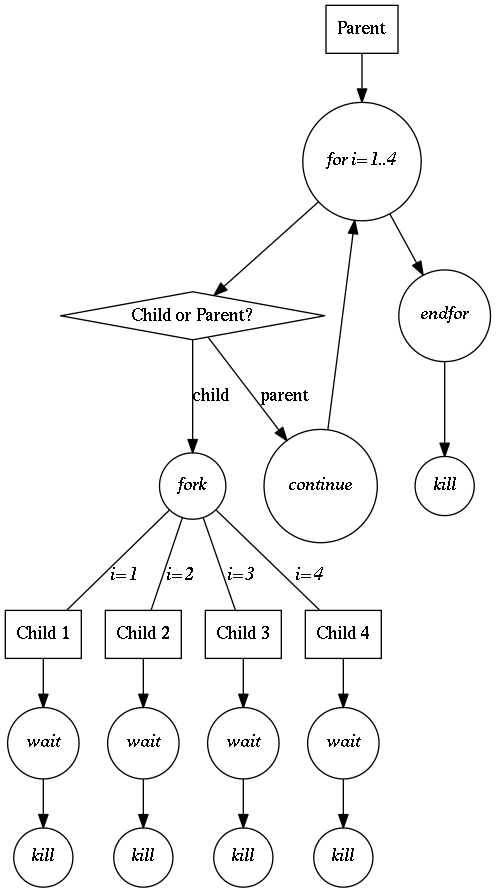
\includegraphics[scale=0.4]{graphs/p2.png}}
\end{figure}

É possível ver que, assim que criam-se todos os processos com |fork| nas quatro
iterações, o processo pai termina sua execução. Os processos filhos tem sua paternidade
automaticamente movida para o processo |init| pelo sistema operacional, o que guarante
que os processos continuem rodando. Assim que cada um acabar sua execução, a memória de cada
processo é liberada. Todos os processos filhos são criados pelo processo pai original.

\end{document}
